\section{Results}
\label{results}

\todo{Describe the results better}

Our aim in the results is to show:
\begin{itemize}
\item The characteristics of the model
\item The results of testing our hypothesis, namely that cupivacaine
  blocks $I_2poreK$, leading to changes in the RMP, leading to changes
  in the volume regulation (which concomitantly leads to changes in
  signaling and potentially apoptosis, or changes therein)
\end{itemize}

These two portions of the results can be presented as two main
categories: ``model-revealing figures'' and ``Hypothesis Figures''.

\subsection{Model-revealing Figures}
In this case, we will present a story which allows us to explain
results of the model and the physiological rationale/relevance of each
component. Simulations for this portion will include both
steady-state, voltage-clamped experiments to show time-independent
behavior, as well as time-dependent currents traces where
applicable. A reasonable voltage range is that used by R. Clark in his
experiments, -130 to +100 mV. An approximate figure list follows.

\begin{itemize}
\item Overall cell behavior: Model schematic. IV curves.
\item Background currents: Input resistance, IV curves, the membrane itself.
\item Pumps and exchanger currents and evolving concentrations: IV
  curves, current traces, concentrations over time, pH versus volume
  (Lewis, et al) -- this shows us how the chondrocyte accounts for
  osmolarity, how we keep track of it.
\item Potassium currents: show all aspects of time-dependent current,
  $I_{kur}$, show main conductances, i.e. $I_{Ca-act K}$ (BK), explain
  basis for RMP
\end{itemize}

\subsection{Hypothesis Figures}
\begin{itemize}
\item Bup. block as initially based on Bob's experiments.
\item 10 percent, 25 percent, 50 percent, 75 percent, 100 percent, and
  perhaps more levels of blockage of $I_{K-2pore}$ conductance
\item Investigate effects on RMP.
\item What adjusts itself in response? Currents? Present these
    currents/concentrations with respect to control.
\item Look specifically at changes in $pH_i$, and link this to volume
  regulation, based on simple formalism from Lewis et al. Creates some
  speculation re: mechanisms that will be interesting and useful for
  Discussion.
\end{itemize}

\begin{figure}
  \centering
  \subfloat{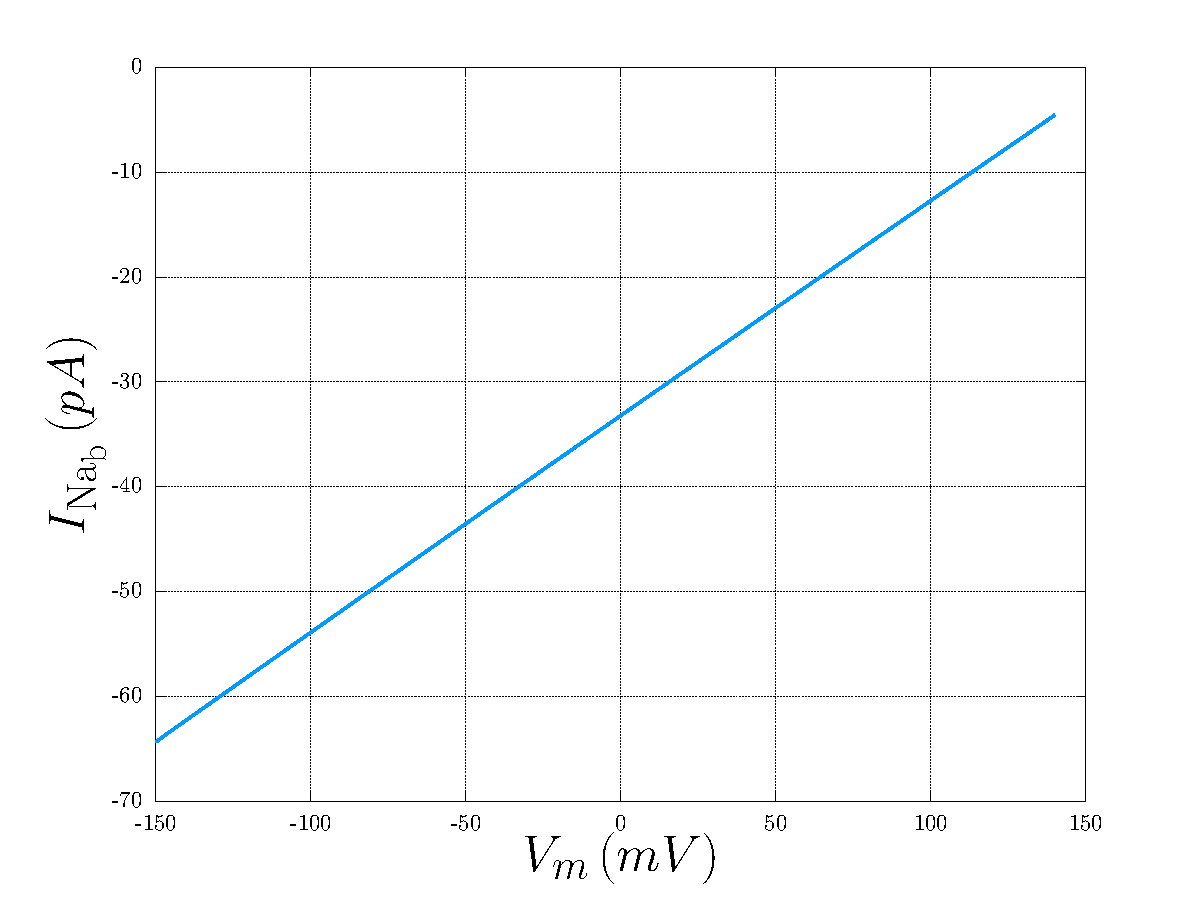
\includegraphics[width=0.38\textwidth]{../results/pdf/V-I_Na_b.pdf}}
  \subfloat{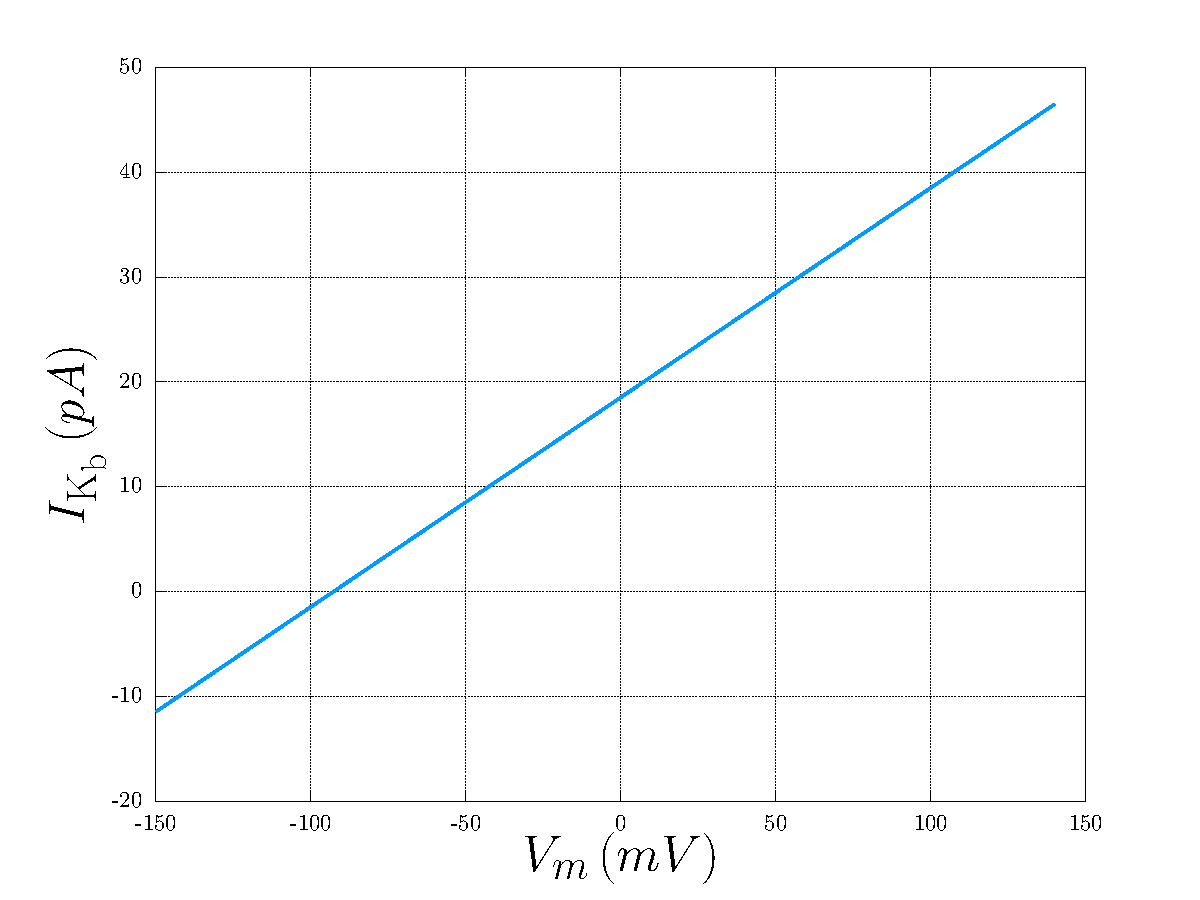
\includegraphics[width=0.38\textwidth]{../results/pdf/V-I_K_b.pdf}}\\
  \subfloat{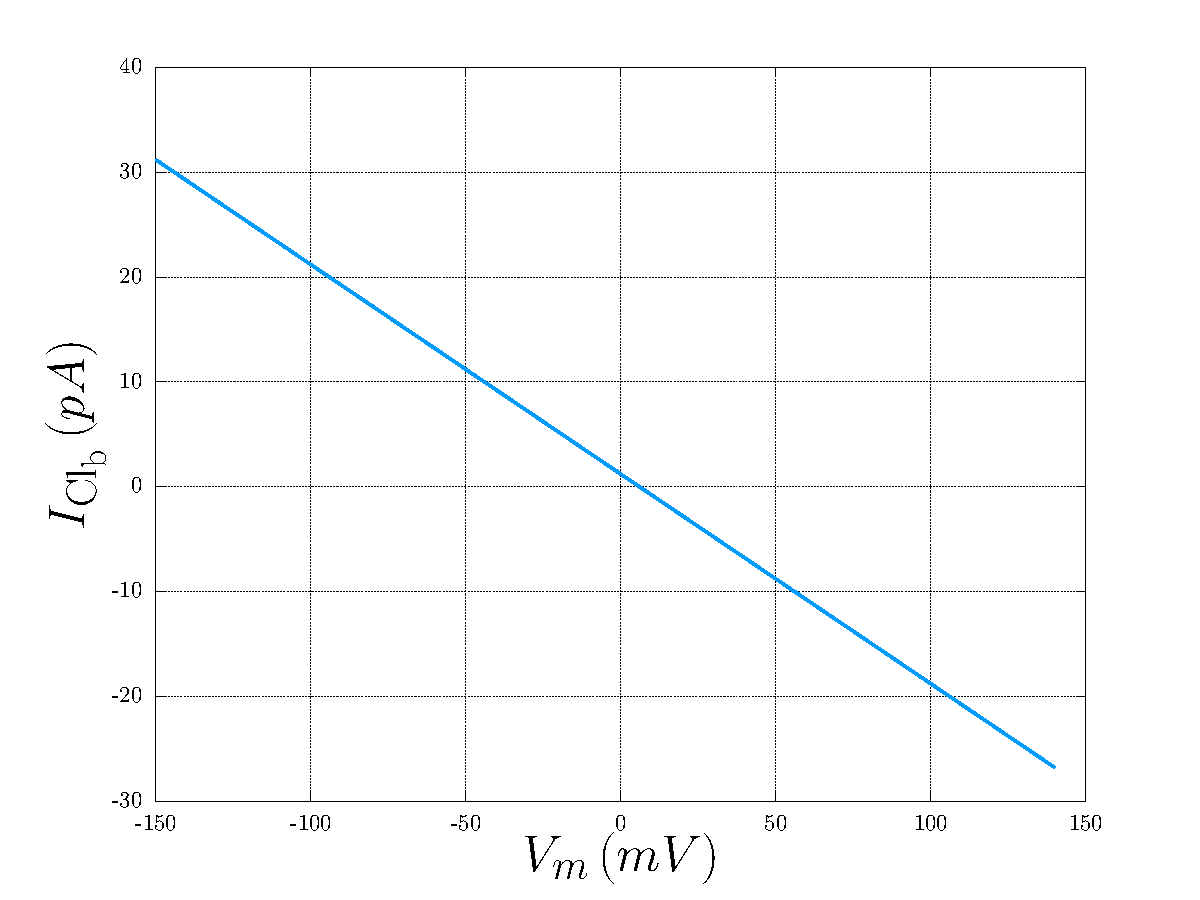
\includegraphics[width=0.38\textwidth]{../results/pdf/V-I_Cl_b.pdf}}
  \subfloat{\hspace{0.38\textwidth}}
  \caption{The background currents (V-I).}
  \label{fig:background-currents-vi}
\end{figure}

\begin{figure}
  \centering
  \subfloat{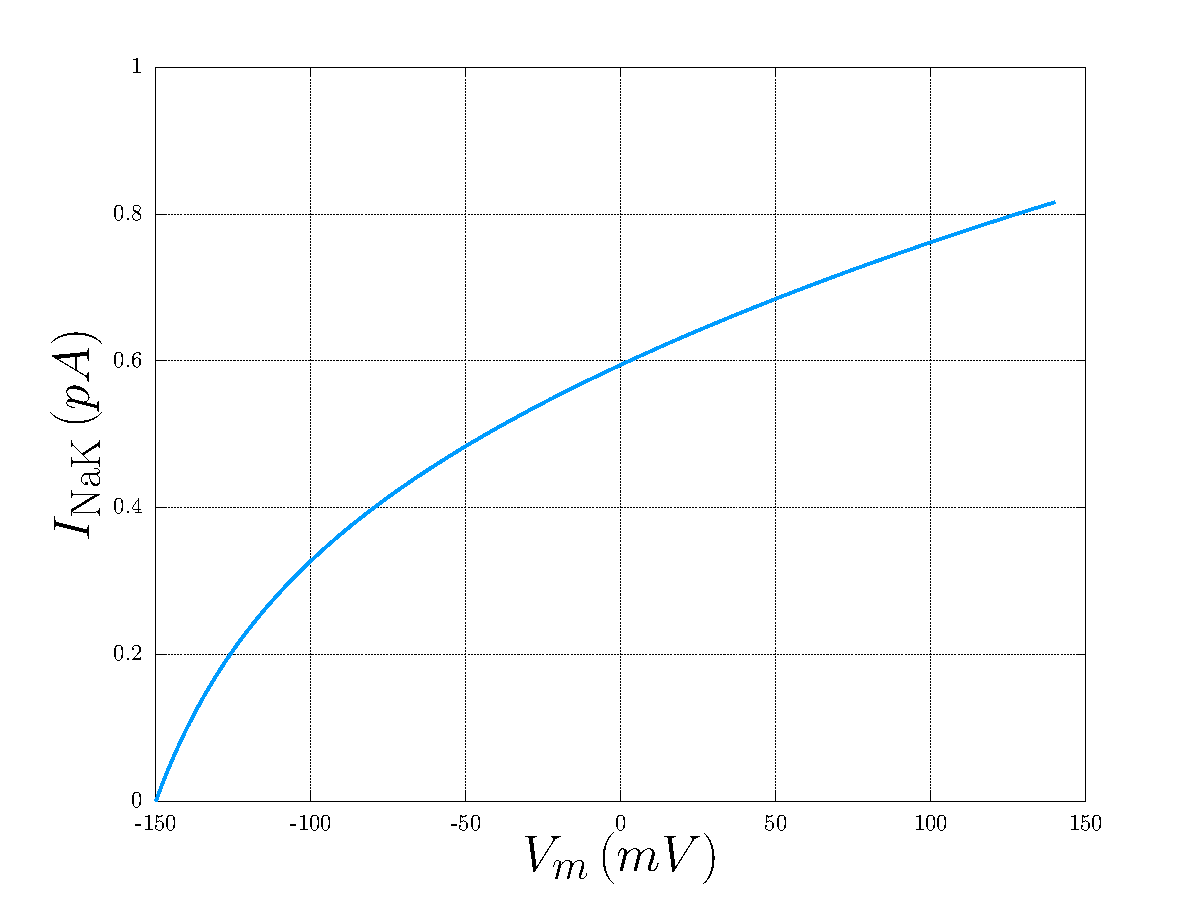
\includegraphics[width=0.38\textwidth]{../results/pdf/V-I_NaK.pdf}}
  \subfloat{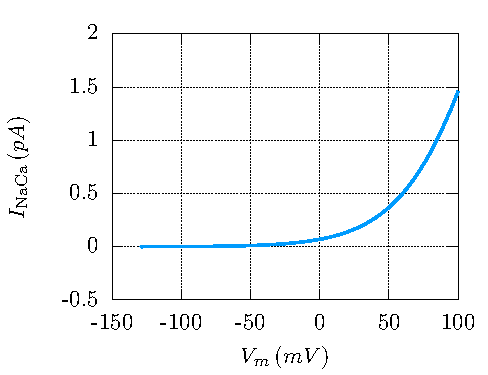
\includegraphics[width=0.38\textwidth]{../results/pdf/V-I_NaCa.pdf}}\\
  \subfloat{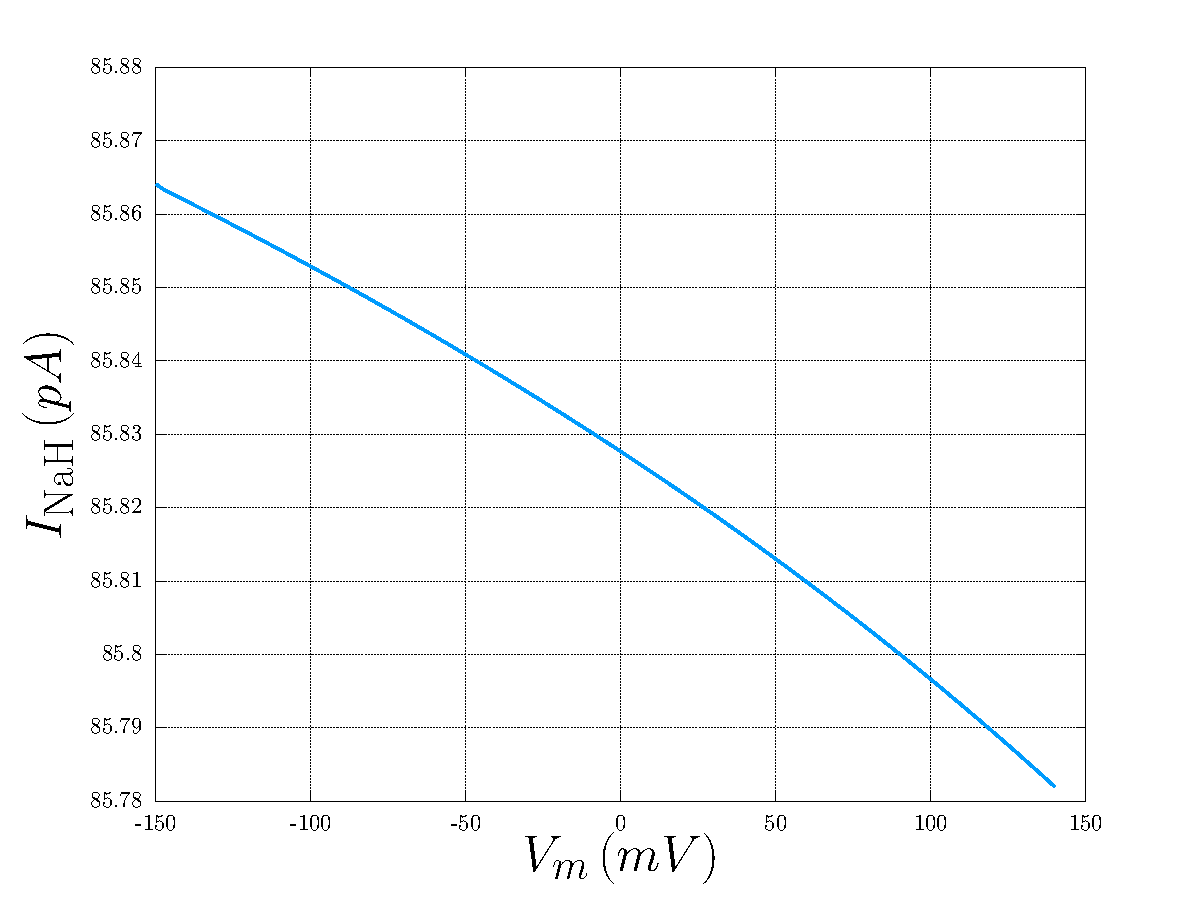
\includegraphics[width=0.38\textwidth]{../results/pdf/V-I_NaH.pdf}}
  \subfloat{\hspace{0.38\textwidth}}
  \caption{The different pumps and exchanger currents (V-I).}
  \label{fig:pumps-and-exchangers-vi}
\end{figure}


\begin{figure}
  \centering
  \subfloat{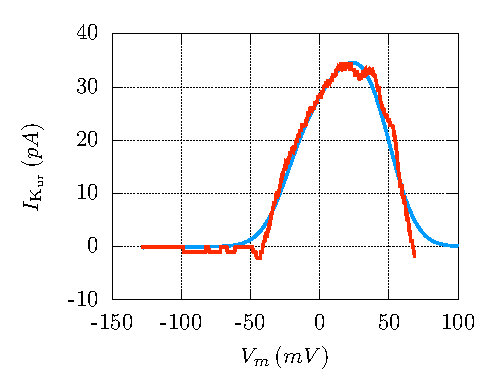
\includegraphics[width=0.38\textwidth]{../results/pdf/V-I_K_ur.pdf}}
  \subfloat{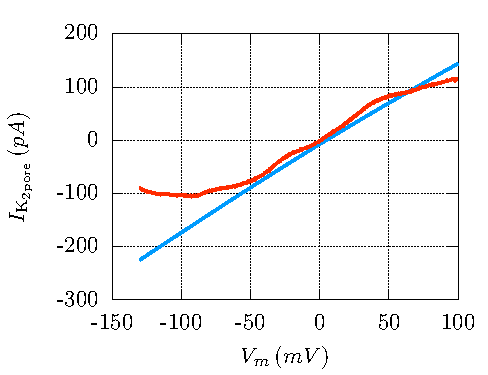
\includegraphics[width=0.38\textwidth]{../results/pdf/V-I_K_2pore.pdf}}\\
  \subfloat{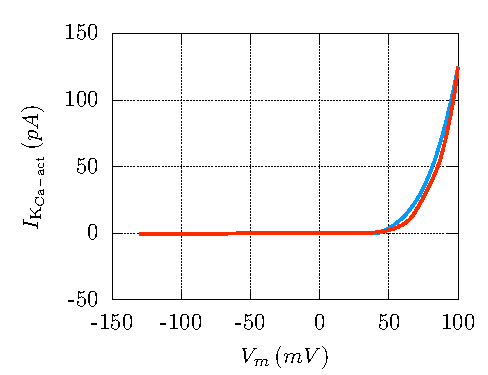
\includegraphics[width=0.38\textwidth]{../results/pdf/V-I_K_Ca_act.pdf}}
  \subfloat{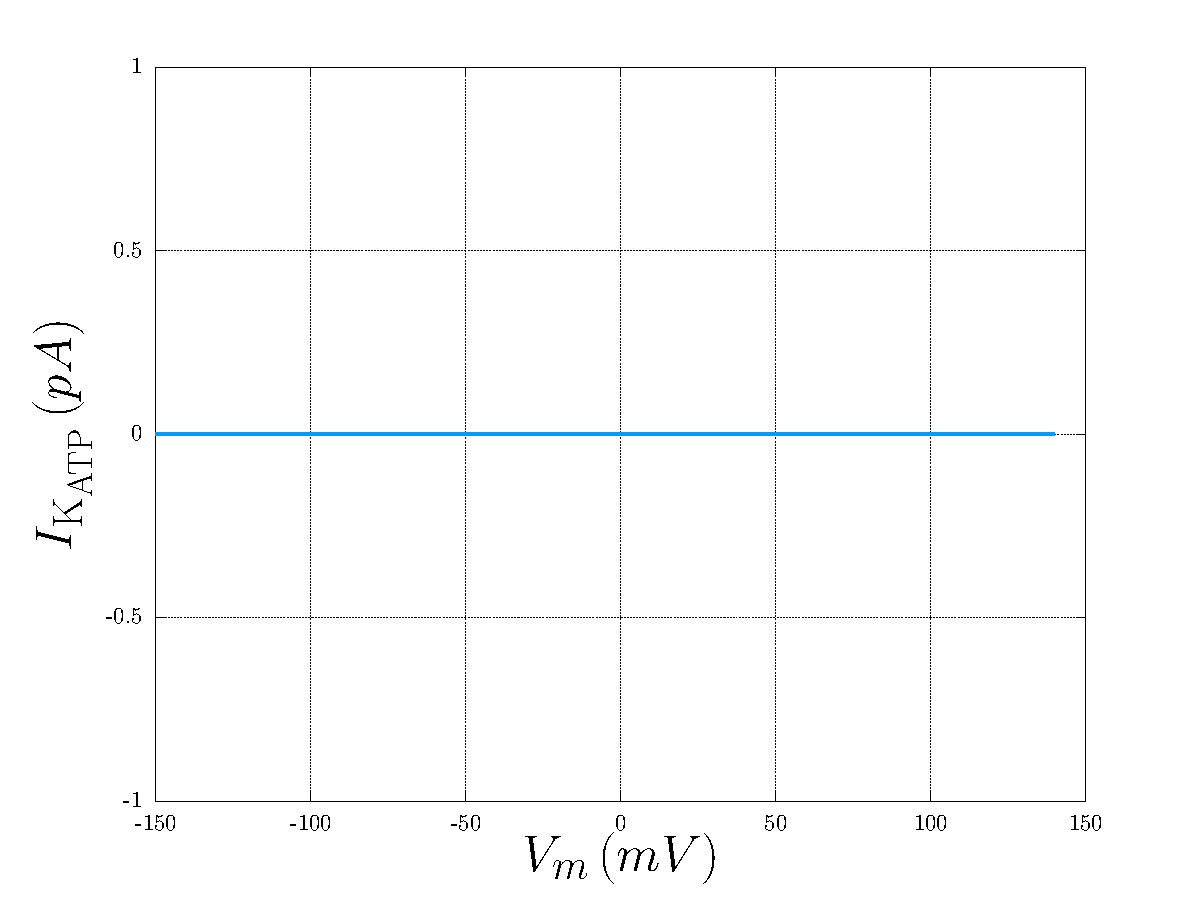
\includegraphics[width=0.38\textwidth]{../results/pdf/V-I_K_ATP.pdf}}
  \caption{The other potassium currents (V-I).}
  \label{fig:potassium-currents-vi}
\end{figure}

% \begin{figure}
%   \centering
%   \includegraphics[width=0.8\textwidth]
%   {../results/pdf/20110506/potassium_currents-vi}
%   \caption{The other potassium currents (steady-state).}
%   \label{fig:potassium-currents-vi}
% \end{figure}

% \begin{figure}
%   \centering
%   \includegraphics[width=0.8\textwidth]
%   {../results/pdf/other_currents-vi}
%   \caption{All other currents (currently turned off or not implemented).}
%   \label{fig:other-behaviour-vi}
% \end{figure}

% \begin{figure}
%   \centering
%   \includegraphics[width=0.8\textwidth]
%   {../results/pdf/20110506/concentrations}
%   \caption{Long-term evolution of the concentrations.}
%   \label{fig:concentrations}
% \end{figure}


% \begin{figure}
%   \centering
%   \includegraphics[width=0.8\textwidth]
%   {../results/pdf/20110506/potassium_currents-ti}
%   \caption{Long-term evolution of the potassium currents.}
%   \label{fig:potassium-currents-ti}
% \end{figure}

% \begin{figure}
%   \centering
%   \includegraphics[width=0.8\textwidth]
%   {../results/pdf/20110506/membrane_behaviour-vi}
%   \caption{Overall steady-state model behaviour when voltage is ramped.}
%   \label{fig:overall-behaviour-vi}
% \end{figure}

% \begin{figure}
%   \centering
%   \includegraphics[width=0.8\textwidth]
%   {../results/pdf/20110506/membrane_behaviour-tv}
%   \caption{Long term evolution of the membrane voltage.}
%   \label{fig:overall-behaviour-tv}
% \end{figure}

\todo{Add some plots from hypothesis tests}

% Local Variables:
% TeX-master: "chondrocyte-model"
% mode: latex
% mode: flyspell
% End:
